

Since there are insufficient boundary conditions to completely define a dislocation's atomic configuration with even four parameters, the energy of the dislocation is the only way to identify a correct or true configuration. Hence we must characterise the energy of atomic configurations. One method to calculate the energy is to try and replicate the model based on elastic energy in the two half crystals and misalignment energy across the slip plane. There is also the opportunity to calculate the full strain tensor and along with single crystal elastic constants the effects of elastic anisotropy can be taken into account. 

Another would be to use empirical potentials similar to those used in molecular dynamics, allowing the exploration of dislocation properties in materials that are not well modelled by elasticity or where more can be learned by other methods. Ionic solids or compound semiconductors are examples of materials where more physical insight is possible with interatomic potentials that relate more closely to the nature of the crystal chemistry than elastic constants. 



The first approach builds on the original approach of \citet{Peierls1940} and \citet{Nabarro1947} and explains how the dislocation is stable due to a balancing of two forces. There is a force that attempts to spread the dislocation out into a planar defect, which arises due to the elastic stored energy in the bonds either side of the slip plane. The elastic energy would be zero in the case of a planar defect, i.e.\ an infinitely wide dislocation. Another force tends to decrease the dislocation width, arising from the misfit or misalignment across the slip plane. The misalignment energy would be a maximum for the planar defect where the entire slip plane is misaligned and would decrease monotonically as the width decreases.

Using an elastic model to find the energy has a number of advantages. A two dimensional model is sufficient since if the  condition of plane strain can be applied. If elastic theory can be applied at the scale of the unit cell then displacements need only be considered between unit cells rather than within them, which simplifies the model considerably.

\subsection{Strain energy}

The elastic energy can be easily calculated for a small volume if the strain and the elastic tensor is known. A good discussion of tensors and elasticity is given by \citet{kelly_knowles2012chapter5_tensors,kelly_knowles2012chapter6_stress_strain} and a discussion of elasticity in the context of dislocation theory is given by \citet{hirth_lothe1982elasticity}. The salient results are drawn together here.

Hooke's Law can be written as a tensor relationship using the Einstein summation convention:
\begin{equation}
\sigma_{ij} = c_{ijkl} \epsilon_{kl}
\end{equation}
where $\sigma_{ij}$ is the stress tensor, $c_{ijkl}$ is the elastic tensor defining the properties of the material and $\epsilon_{kl}$ is the strain tensor. Strain is defined, for $i=j$, by
\begin{equation}
\epsilon_{ii} = \frac{\partial u_i}{\partial x_i}
\end{equation}
and for $i\neq j$ by
\begin{equation}
\epsilon_{ij} = \frac{1}{2} \left( \frac{\partial u_i}{\partial x_j} + \frac{\partial u_j}{\partial x_i} \right).
\end{equation}
%In Voigt notation the equation can be written
%\begin{equation}
%\sigma_i = c_{ij} \epsilon_{j}
%\end{equation}
%where 
%\begin{equation}
%\sigma_i = \begin{bmatrix}
%\sigma_{11} \\
%\sigma_{22} \\
%\sigma_{33} \\
%\sigma_{23} \\
%\sigma_{31} \\
%\sigma_{12} 
%\end{bmatrix}
%\qquad\qquad
%\epsilon_i = \begin{bmatrix}
%\epsilon_{11} \\
%\epsilon_{22} \\
%\epsilon_{33} \\
%\gamma_{23} \\
%\gamma_{31} \\
%\gamma_{12} 
%\end{bmatrix}
%\end{equation}
%This allows the reduction of the $3\times3\times3\times3$ tensor $c_{ijkl}$ to a $6\times6$ matrix $c_{ij}$. Note that to preserve the symmetry across the leading diagonal in $c_{ij}$ the strain components for $i\neq j$ are defined by $\gamma_{ij} = 2 \epsilon_{ij}$.
If Hooke's law holds then the stored elastic energy per unit volume is
\begin{equation}
u_{\text{elastic}} =\, ^{1}\!/_{2}\, \sigma_{ij} \epsilon_{ij} =\, ^{1}\!/_{2}\, c_{ijkl} \epsilon_{ij} \epsilon_{kl}.
\end{equation}
Hence to find the elastic energy we must evaluate \({\partial u_i}/{\partial x_j}\) for $i, j = 1, 2, 3$.
Assuming a primitive orthogonal lattice, estimating the components of strain is not difficult. The  condition of plane strain constrains $\epsilon_{ij} = 0$ for $i\, \text{or}\, j=3$. In the $1$--$2$ (or $x$--$y$) plane the strains can be identified from the vectors between neighbouring unit cells. For simplicity a primitive lattice is assumed and these vectors can be conceived of as bonds.

For this simple case two bonds are identified for each atom, one to the nearest neighbour in the $x$~direction and one to the nearest neighbour in the $y$~direction as shown in \autoref{fig:bonds}. The simplest estimate of the stress components is
\begin{alignat}{2}\label{eqn:estimate_strains}
\left. \frac{\partial u_x}{\partial x}\right|_i &= \frac{\mathbf{p}_i \cdot \mathbf{\hat{i}}}{b} &\qquad\qquad
\left. \frac{\partial u_x}{\partial y}\right|_i &= \frac{\mathbf{q}_i \cdot \mathbf{\hat{i}}}{d} \nonumber\\
\left. \frac{\partial u_y}{\partial y}\right|_i &= \frac{\mathbf{q}_i \cdot \mathbf{\hat{j}}}{d} &
\left. \frac{\partial u_y}{\partial x}\right|_i &= \frac{\mathbf{p}_i \cdot \mathbf{\hat{j}}}{b}
\end{alignat}


\begin{figure}
\centering
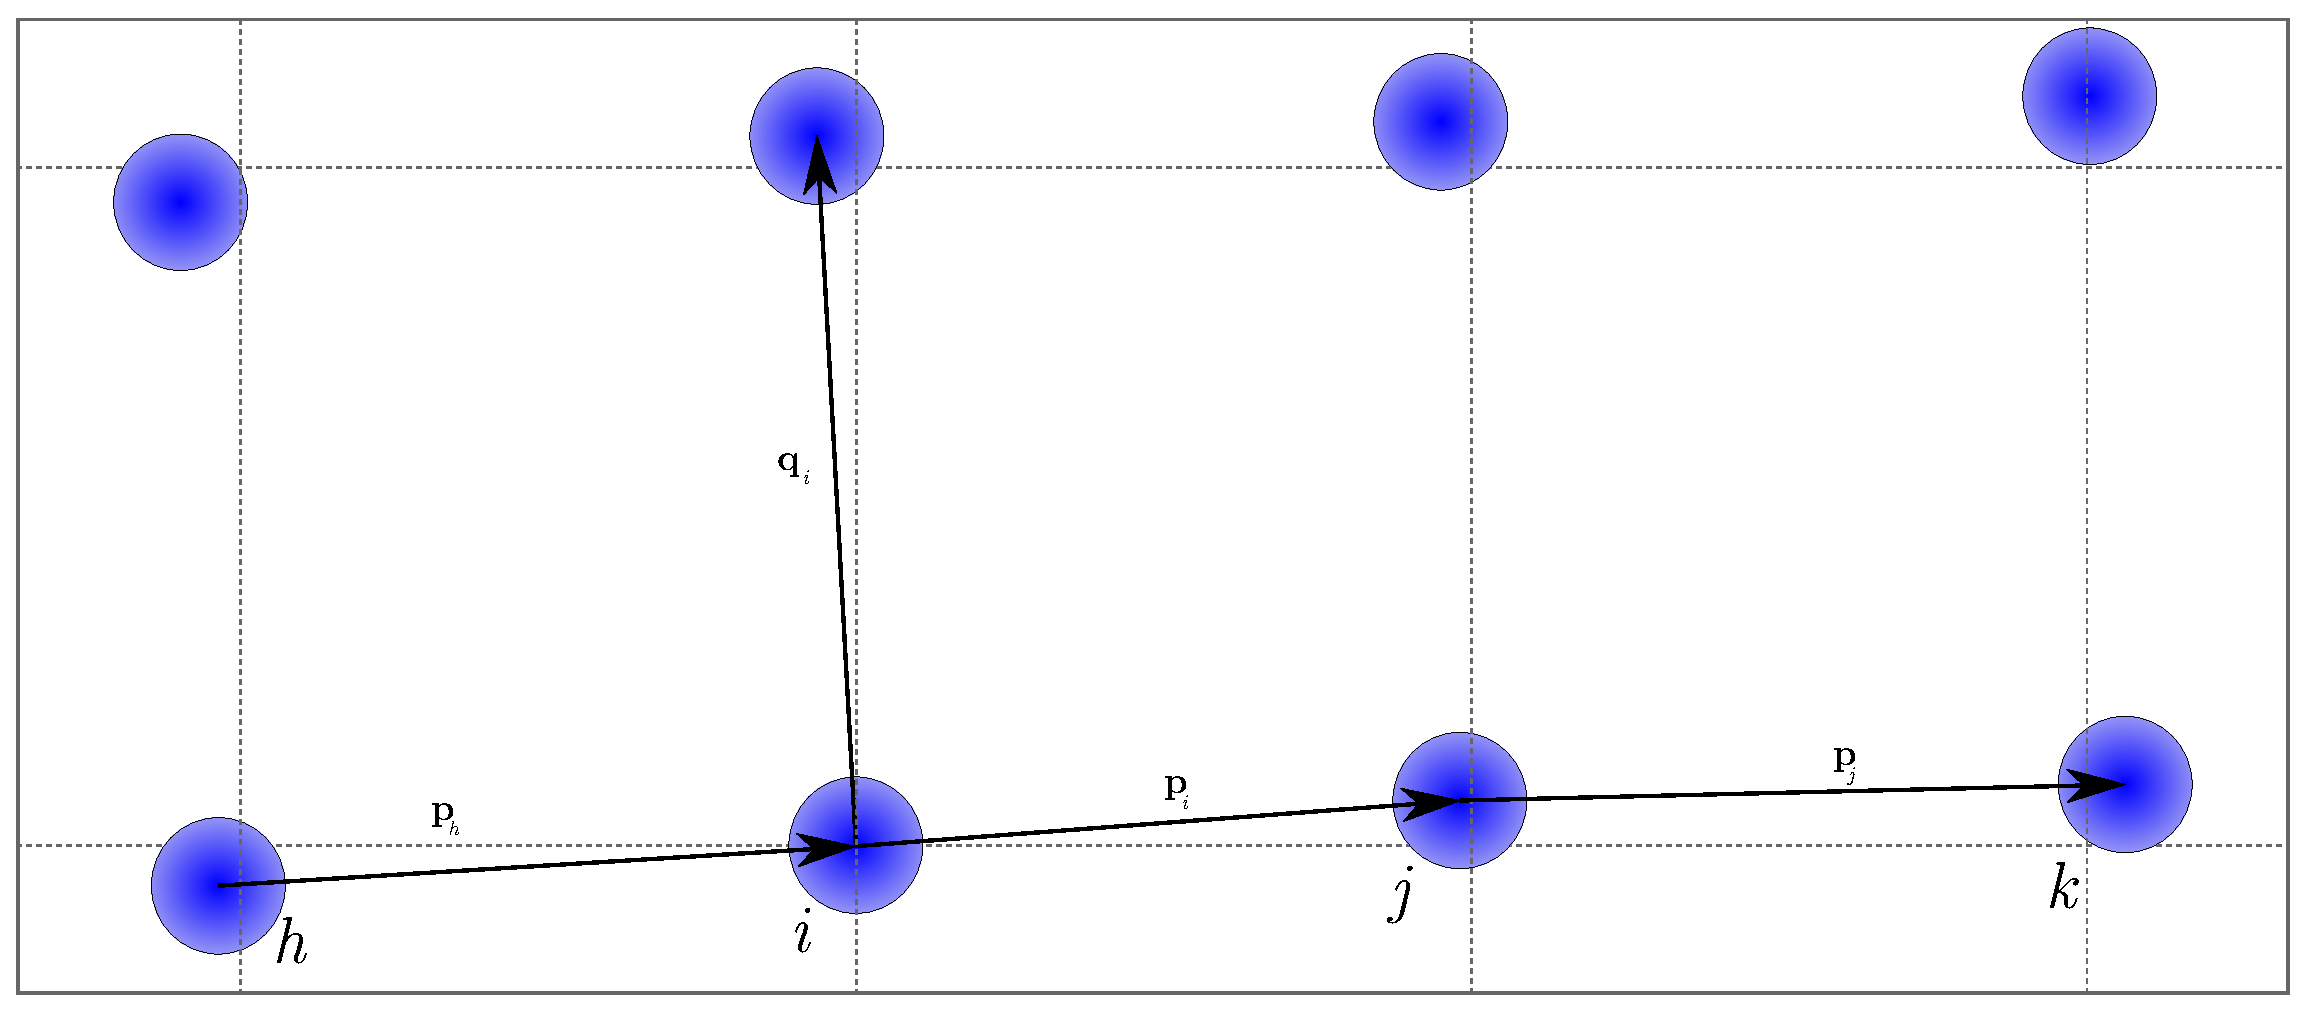
\includegraphics[width=\textwidth]{bonds}
\caption[Strained bonds in a dislocated crystal.]{The bonds that are considered for the $i$th atom in a region of crystal away from the slip plane; there is one bond to the nearest neighbour in the positive $x$~direction, $\mathbf{p}_i$, and one to the nearest neighbour in the positive $y$~direction, $\mathbf{q}_i$, to avoid double counting.\label{fig:bonds} }
\end{figure}





However there is a problem with this formulation. This assumes that every bond would, in equilibrium, be parallel to either the $x$ or the $y$ axis. This assumption is valid for the original Peierls model in which only displacements parallel to the $x$ direction were considered but the logarithmic term here represents a change in lattice orientation with position. 

Addressing this requires some estimate of the local lattice orientation. The logarithmic term in \autoref{eqn:displacements}, representing the bending of the lattice, means that far from the dislocation core the lattice can be tilted to a large angle with respect to the slip direction at the core. If the same reference axes are used everywhere, this bending results in an ever increasing strain, and therefore ever increasing strain energy away from the core. Using a local lattice orientation as the reference frame to calculate the strain means that strains will be largest near the core, as expected.


There are many possible ways of estimating the local lattice orientation. One possible method is to take the average of the neighbouring bonds so for the atom labelled $i$ shown in \autoref{fig:bonds} the ideal orientation of $\mathbf{p}_i$ would be  parallel to $(\mathbf{p}_h + \mathbf{p}_j)$. The ideal orientation for $\mathbf{q}_i$ can be taken to be at \SI{90}{\degree} to this. Therefore $\mathbf{\hat{i}}$ and $\mathbf{\hat{j}}$ in \autoref{eqn:estimate_strains} can be replaced with 
\begin{align}
\mathbf{\hat{i}}' &= \frac{(\mathbf{p}_h + \mathbf{p}_j)}{|\mathbf{p}_h + \mathbf{p}_j|} \nonumber \\
\mathbf{\hat{j}}' &= {\mathbf{\hat{i}}' \times \mathbf{\hat{k}}}
\end{align}
and the strain tensor can be calculated for each atom/unit cell, and hence the strain energy for each unit cell.




\subsection{Misalignment energy}


At the slip plane the method above will break down. For an atom immediately below the slip plane the identification of the nearest neighbour above the slip plane can be ambiguous, or can leave some atoms multiply bonded and others unbonded, the nearest neighbour will also change as the dislocation moves. \autoref{fig:slip_plane} shows an possible configuration around a dislocation core that would result in this kind of problem. Considering the atom $m$, it can be seen that it is further from both atom $i$ and atom $j$ than their other neighbours, $l$ and $n$, and so atom $m$ would be unbonded in a simple nearest neighbour model. The atom $n$ might be bonded twice in such a model.

A less arbitrary method is to use the initial positions and assume that the $i$th atom can be bonded to two atoms in the layer above the slip plane. Since initially the horizontal spacing between atoms is $b$ for all atoms the two atoms must be within an interval $x_i^0 - b < x \leq x_i^0 + b$, bonds can be identified as shown in \autoref{fig:slip_plane_initial_positions}. The energy of the two bonds is averaged to avoid a double counting error.

\begin{figure}
\centering
\begin{subfigure}{\textwidth}
\centering
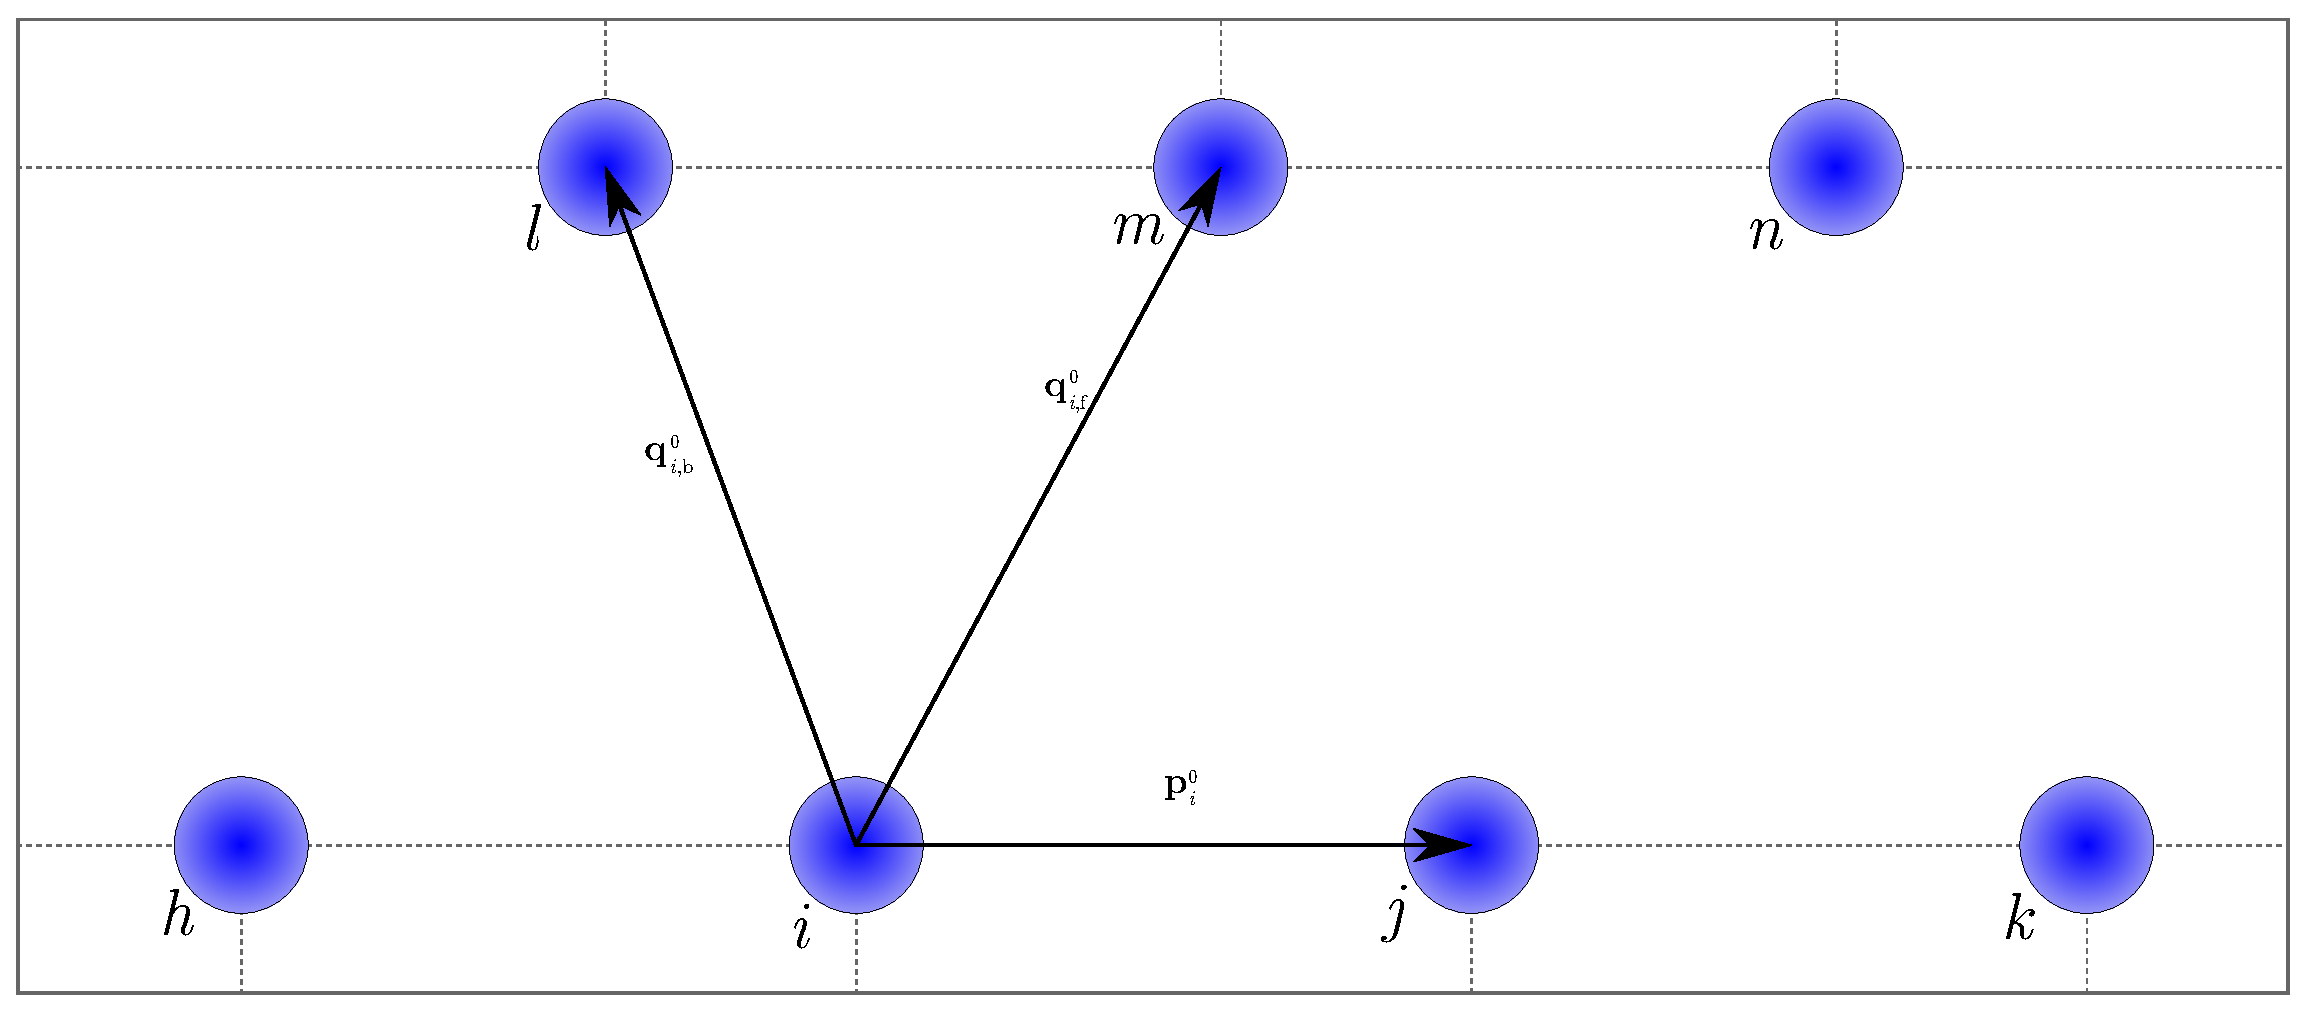
\includegraphics[width=\textwidth]{initial_slip_plane_bonds}
\caption{The initial positions of atoms either side of the slip plane.\label{fig:slip_plane_initial_positions}.}
\end{subfigure}
\par\medskip
\begin{subfigure}{\textwidth}
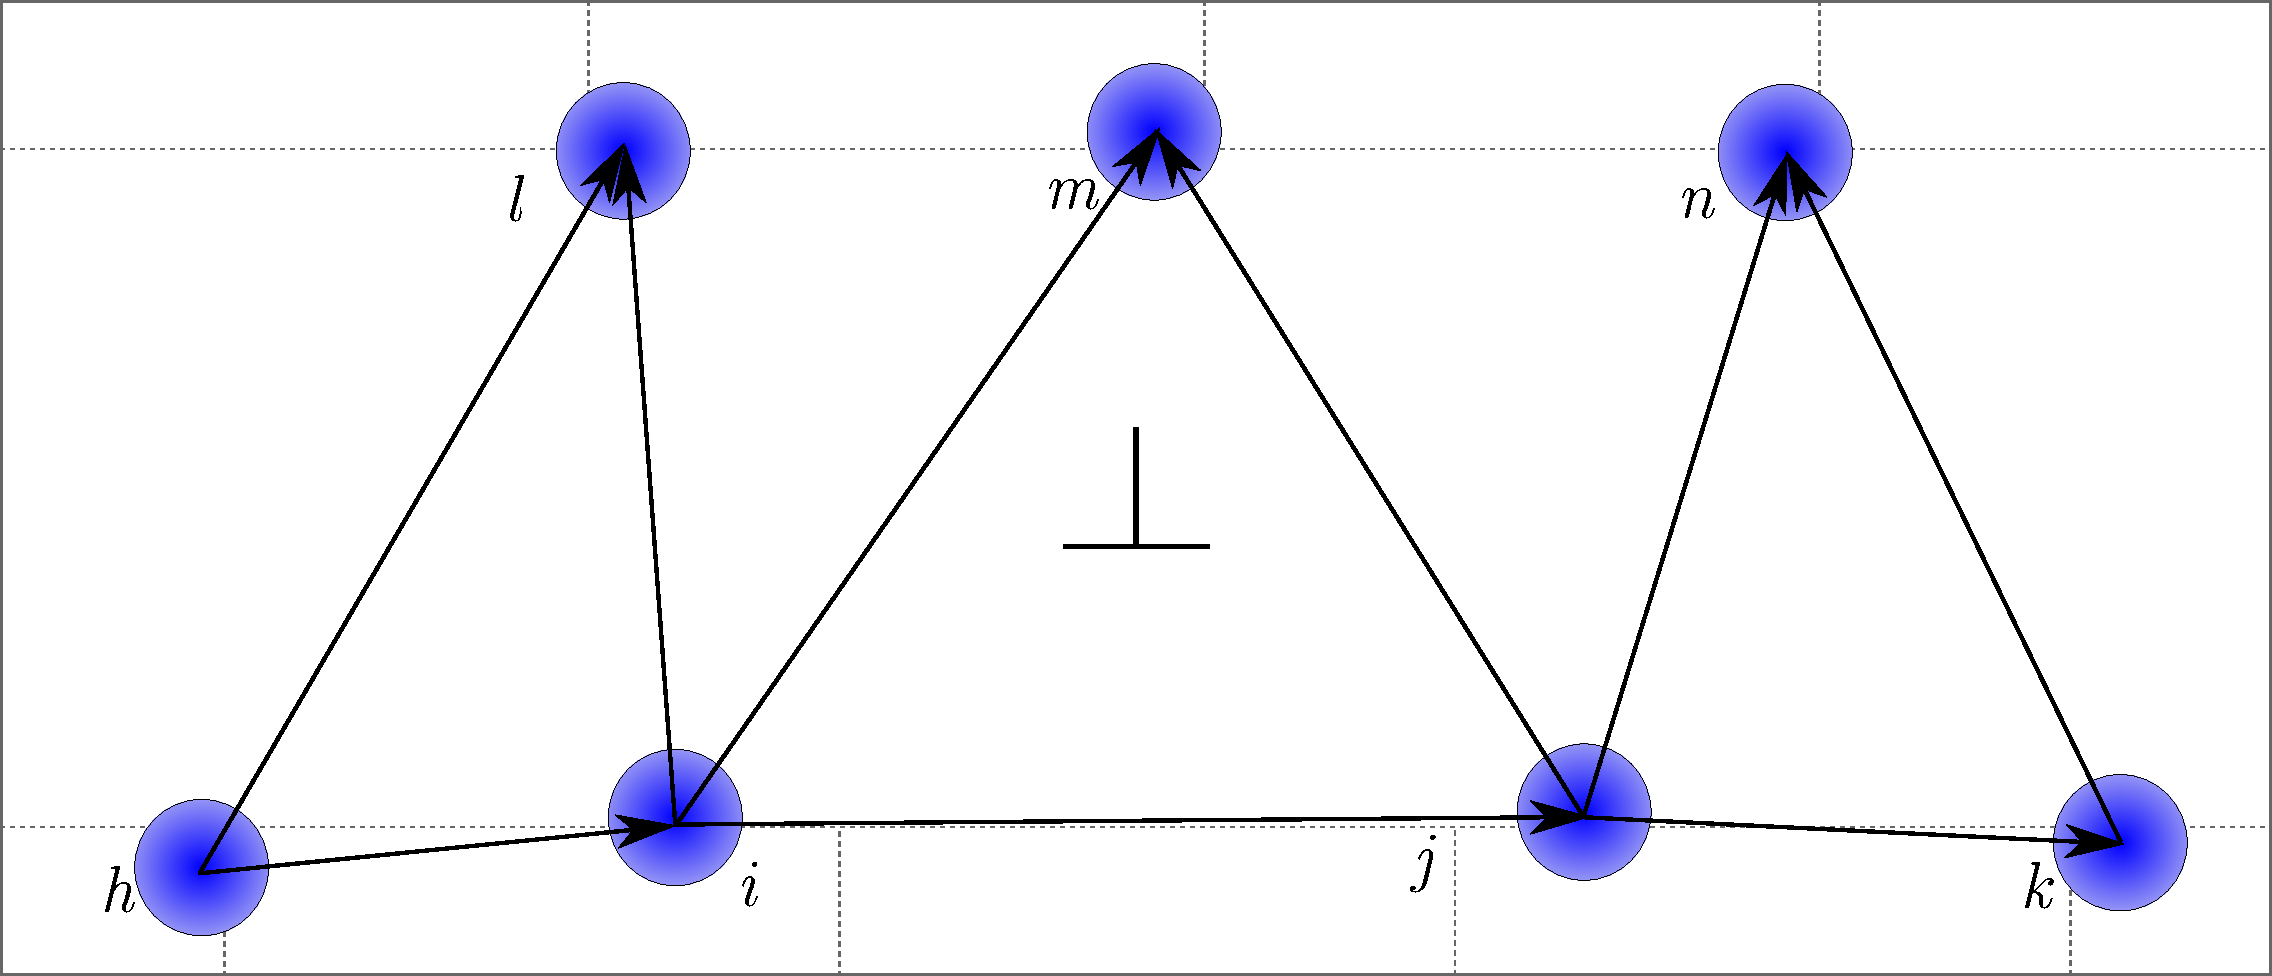
\includegraphics[width=\textwidth]{slip_plane_bonds}
\caption{The final positions of the atoms either side of the slip plane.\label{fig:slip_plane_final_positions}}
\end{subfigure}
\caption[Misaligned bonds across the slip plane.]{The slip plane before and after the application of the displacement field in the vicinity of the dislocation core. If we consider only nearest neighbours then the atom labelled $m$ would be unbonded while others, like $n$ would be bonded twice. Ambiguities can also arise when neighbours are equidistant and the neighbours would also change as the dislocation moved using a nearest neighbours model. Instead the two nearest neighbours across the slip plane are considered, as shown this results in a forward bond and a backward bond. Notice the changing orientation of the slip plane in the dislocated crystal.\label{fig:slip_plane}}
\end{figure}


There are several methods to calculate the energy of the misaligned bonds. The simplest is to use the Frenkel approximation which, for an isotropic elastic material is 
\begin{equation}
U_i^\text{mis} = \frac{Gb^2}{4\pi^2} \left[\frac{d}{b}\right] \left[ 1 - \cos \left( \frac{2 \pi \phi}{d} \right) \right]
\end{equation}
which in terms of single crystal elastic constants takes $G=C_{66}$ (in Voigt notation see \cite{kelly_knowles2012chapter6_stress_strain}). The $66$ term is used if the elastic tensor is in the frame of reference of  the slip system, with the $1$ axis parallel to the slip direction, the $2$ axis parallel to the slip plane normal and the $3$ axis parallel to the line vector. $C_{66}$ is thus always the relevant stiffness constant regardless of the material symmetry.

A more complete method for the calculation of the energy is to use the generalised stacking fault energy. Density functional theory can be used to calculate the energy of a stacking fault at an arbitrary misalignment. This is calculated by applying a displacement to two half crystals in a DFT simulation with periodic boundary conditions which introduces two opposing planar faults. The displacement is applied along the Burgers vector and the atoms are allowed to relax perpendicular to that displacement. Although the displacement field does not include any lateral motion (i.e. parallel to the dislocation line), allowing the DFT simulation of the stacking faults to relax laterally means that the energetic implications of lateral motion are included in the misalignment potential, although with an implicit assumption that the strains along the line vector do not extend beyond the slip plane. 

The energy changes with respect to a perfect crystal were considered and fitted with a simple empirical function:
\begin{equation}
\gamma(\phi) = \sum^{M}_{m=1} C_m \left[ 1 - \cos \left( \frac{2m\pi \phi}{b} \right) \right]
\end{equation}
where $\phi$ is the misalignment in the same units as the Burgers vector $b$, $m$ is an integer from \num{1} to $M$ and $C_m$ are coefficients fitted by a least-squares method to the energies calculated by DFT for different values of $\phi$. This is in units of \si{\joule\per\square\meter}, so a factor of $b$ must be applied to convert to a line energy in \si{\joule\per\meter}.


%%%%%%%%%%%%%%%%%%%%%%%%%%%%%%%%%%%%%%%%%%%%%%%%%%%%%%%%%%%%%%%5555%%%%%%%%%%%%%%%%%%%%%%%%%%%%%%%%%%%%%%%%%






%%%%%%%%%%%%%%%%%%%%%%%%%%%%%%%%%%%%%%%%%%%%%%%%%%%%%%%%%%%%%%%%%%%%%%%%%%%%%%%%%%%%%%%%%%%%%%%%%%%




\subsection{Empirical potentials}

Some materials can be described in a more physically insightful way than linear elasticity; as described in \autoref{sec:empirical_potentials}, empirical potentials have been developed for the field of molecular dynamics to be computationally convenient while at the same time approximating reality to a sufficient degree to gain insight into a system \cite{martinez2013}. Such potentials are usually fitted to measured properties such as lattice energies and elastic constants.

One way to incorporate such potentials into the Peierls model described here is to write a simple Python implementation of the potentials using the SciPy and NumPy packages and associated tools \cite{Numpy2011,IPython2007,Millman2007,SciPy2001}; another way is to use the Atomic Simulation Environment \cite{ASE2017} or the Python interface to the LAMMPS software package \cite{Plimpton1995,LAMMPS_web}.



The ionic solids were investigated using the Lennard-Jones potential:
\begin{equation}
\phi_{ij}(r_{ij}) = 4\epsilon_{ij} \left[ \left( \frac{\sigma_{ij}}{r_{ij}}\right)^{12}-     \left( \frac{\sigma_{ij}}{r_{ij}}\right)^6   \right]
\end{equation}
where $\epsilon_{ij}$ is the depth of the energy well and $\sigma_{ij}$ is the radius at which the energy is equal to zero or in the A--B form:
\begin{equation}
\phi_{ij}(r_{ij}) = \frac{A_{ij}}{r_{ij}^{12}} - \frac{B_{ij}}{r_{ij}^{6}}
\end{equation}
where $A_{ij} = 4\epsilon_{ij}\sigma_{ij}^{12}$ and $B_{ij} = 4 \epsilon_{ij} \sigma_{ij}^{6}$. The energy for any two atoms is then 
\begin{equation}
U_{ij}(r_{ij}) = \frac{1}{4\pi\epsilon_0} \frac{q_i q_j}{r_{ij}} + \frac{A_{ij}}{r_{ij}^{12}} - \frac{B_{ij}}{r_{ij}^{6}}
\end{equation}
where $\epsilon_0$ is the permittivity of free space.

The Lennard-Jones potential  has been chosen as a simple way to demonstrate the application of empirical potentials. Fitted parameters are readily available \cite{Mao2014} and the potential is applicable to a class of materials for which the dislocation properties are not fully understood, the alkali halides.



\begin{table}
\centering
  \begin{tabular}{| m{3cm} | d{4} | d{-1} |}
  \hline
   Ion \rule{0pt}{3ex} & \multicolumn{1}{c|}{$\sigma_i$/\si{\angstrom}} & \multicolumn{1}{c|}{$\epsilon_i$/\si{\joule\per\mole}  }\\ \hline
   \ce{Li+} \rule{2ex}{0pt} & 1.715 & 241.25 \\
   \ce{Na+} & 2.497 & 327.44 \\
   \ce{K+} & 3.184 & 494.97 \\
   \ce{Rb+} & 3.302 & 1006.25 \\
   \ce{Cs+} & 3.440 & 2097.44 \\
   \ce{F-} & 3.954 & 27.05 \\
   \ce{Cl-} & 4.612 & 104.68 \\
   \ce{Br-} & 4.812 & 150.46  \\
   \ce{I-} & 5.197  & 176.56 \\
  \hline
  \end{tabular}
\caption[Lennard-Jones parameters.]{\rule[3ex]{0pt}{0pt} Parameters used for Lennard-Jones calculations from \cite{Mao2014}.\label{tab:LJ_params}}
\end{table}


The parameters used for the Lennard-Jones potential are shown in \autoref{tab:LJ_params}. These were fitted to the lattice properties of the solid salts. They are calculated for each ion individually, to best reproduce lattice properties, and must be combined according to Lorentz-Berthelot rules:
\begin{align}
\epsilon_{ij} &= \sqrt[]{\epsilon_i \epsilon_j} \nonumber\\
\sigma_{ij} &= \frac{\sigma_i + \sigma_j}{2}
\end{align}

A simple implementation without modification for computational ease, such as cut off distances, is given in \cite{code} and an example input file is given for LAMMPS in section~\ref{sec:lammps_input}. LAMMPS  input files are described in the LAMMPS documentation \cite{LAMMPS_web}.

\subsection{Optimisation of the dislocation structure}
\label{sec:optimisers}


Given one of the above cases, or a similar one, that provides energy as a function of a small number of parameters, an optimisation routine is required. The original version of this Peierls model \cite{Clegg2006} included a simple binary search to find the width of the dislocation. However for a multi-parameter space this is not applicable.

Fortunately the open source project SciPy includes implementations of a number of optimisers. The one chosen here was the quasi-Newton method of Broyden, Fletcher, Goldfarb, and Shanno \citep{SciPy2001,nocedal2006}, or BFGS. This method uses the first derivative of the energy with respect to the different parameters, and is one of the class of algorithms known as hill-climbing optimisers, which seek a stationary point.

While the derivative of the energy with respect to the parameters is not simple to find, the atomic positions are defined as smooth functions of the input parameters and the energy is (at least likely to be) a smooth function of the atomic positions. Hence the overall behaviour of the energy as a function of the input parameters should be well suited to a gradient based method. The SciPy implementation of the BFGS algorithm includes the ability to approximate the first derivative numerically.

If it is found that the energy function is not well behaved, SciPy also includes the Nelder-Mead simplex algorithm that does not make use of gradient information. This method calculates the objective function, here the energy, at $n+1$ points in parameter space where $n$ is the number of parameters. This defines a ``simplex'', i.e. a triangle in two dimensions, a tetrahedron in three and so on. A search direction is defined along the vector joining the worst of these $n+1$ points and the centroid of the rest, and a small number of point along this line are trialled. The worst point of the initial simplex is then replaced and the process repeated \citep{Nelder1965,Gao2012}.























































